\pdfbookmark{Общая характеристика работы}{characteristic}             % Закладка pdf
\section*{Общая характеристика работы}

\newcommand{\actuality}{\pdfbookmark[1]{Актуальность}{actuality}\underline{\textbf{\actualityTXT}}}
\newcommand{\progress}{\pdfbookmark[1]{Разработанность темы}{progress}\underline{\textbf{\progressTXT}}}
\newcommand{\aim}{\pdfbookmark[1]{Цели}{aim}\underline{{\textbf\aimTXT}}}
\newcommand{\tasks}{\pdfbookmark[1]{Задачи}{tasks}\underline{\textbf{\tasksTXT}}}
\newcommand{\aimtasks}{\pdfbookmark[1]{Цели и задачи}{aimtasks}\aimtasksTXT}
\newcommand{\novelty}{\pdfbookmark[1]{Научная новизна}{novelty}\underline{\textbf{\noveltyTXT}}}
\newcommand{\influence}{\pdfbookmark[1]{Практическая значимость}{influence}\underline{\textbf{\influenceTXT}}}
\newcommand{\methods}{\pdfbookmark[1]{Методология и методы исследования}{methods}\underline{\textbf{\methodsTXT}}}
\newcommand{\defpositions}{\pdfbookmark[1]{Положения, выносимые на защиту}{defpositions}\underline{\textbf{\defpositionsTXT}}}
\newcommand{\reliability}{\pdfbookmark[1]{Достоверность}{reliability}\underline{\textbf{\reliabilityTXT}}}
\newcommand{\probation}{\pdfbookmark[1]{Апробация}{probation}\underline{\textbf{\probationTXT}}}
\newcommand{\contribution}{\pdfbookmark[1]{Личный вклад}{contribution}\underline{\textbf{\contributionTXT}}}
\newcommand{\publications}{\pdfbookmark[1]{Публикации}{publications}\underline{\textbf{\publicationsTXT}}}


{\actuality} Обзор, введение в тему, обозначение места данной работы в
мировых исследованиях и~т.\:п., можно использовать ссылки на~другие
работы~\autocite{Gosele1999161,Lermontov}
(если их~нет, то~в~автореферате
автоматически пропадёт раздел <<Список литературы>>). Внимание! Ссылки
на~другие работы в~разделе общей характеристики работы можно
использовать только при использовании \verb!biblatex! (из-за технических
ограничений \verb!bibtex8!. Это связано с тем, что одна
и~та~же~характеристика используются и~в~тексте диссертации, и в
автореферате. В~последнем, согласно ГОСТ, должен присутствовать список
работ автора по~теме диссертации, а~\verb!bibtex8! не~умеет выводить в~одном
файле два списка литературы).
При использовании \verb!biblatex! возможно использование исключительно
в~автореферате подстрочных ссылок
для других работ командой \verb!\autocite!, а~также цитирование
собственных работ командой \verb!\cite!. Для этого в~файле
\verb!common/setup.tex! необходимо присвоить положительное значение
счётчику \verb!\setcounter{usefootcite}{1}!.

Для генерации содержимого титульного листа автореферата, диссертации
и~презентации используются данные из файла \verb!common/data.tex!. Если,
например, вы меняете название диссертации, то оно автоматически
появится в~итоговых файлах после очередного запуска \LaTeX. Согласно
ГОСТ 7.0.11-2011 <<5.1.1 Титульный лист является первой страницей
диссертации, служит источником информации, необходимой для обработки и
поиска документа>>. Наличие логотипа организации на~титульном листе
упрощает обработку и~поиск, для этого разметите логотип вашей
организации в папке images в~формате PDF (лучше найти его в векторном
варианте, чтобы он хорошо смотрелся при печати) под именем
\verb!logo.pdf!. Настроить размер изображения с логотипом можно
в~соответствующих местах файлов \verb!title.tex!  отдельно для
диссертации и автореферата. Если вам логотип не~нужен, то просто
удалите файл с~логотипом.

\ifsynopsis
Этот абзац появляется только в~автореферате.
Для формирования блоков, которые будут обрабатываться только в~автореферате,
заведена проверка условия \verb!\!\verb!ifsynopsis!.
Значение условия задаётся в~основном файле документа (\verb!synopsis.tex! для
автореферата).
\else
Этот абзац появляется только в~диссертации.
Через проверку условия \verb!\!\verb!ifsynopsis!, задаваемого в~основном файле
документа (\verb!dissertation.tex! для диссертации), можно сделать новую
команду, обеспечивающую появление цитаты в~диссертации, но~не~в~автореферате.
\fi

% {\progress}
% Этот раздел должен быть отдельным структурным элементом по
% ГОСТ, но он, как правило, включается в описание актуальности
% темы. Нужен он отдельным структурынм элемементом или нет ---
% смотрите другие диссертации вашего совета, скорее всего не нужен.

{\aim} данной работы является \ldots

Для~достижения поставленной цели необходимо было решить следующие {\tasks}:
\begin{enumerate}[beginpenalty=10000] % https://tex.stackexchange.com/a/476052/104425
  \item Исследовать, разработать, вычислить и~т.\:д. и~т.\:п.
  \item Исследовать, разработать, вычислить и~т.\:д. и~т.\:п.
  \item Исследовать, разработать, вычислить и~т.\:д. и~т.\:п.
  \item Исследовать, разработать, вычислить и~т.\:д. и~т.\:п.
\end{enumerate}


{\novelty}
\begin{enumerate}[beginpenalty=10000] % https://tex.stackexchange.com/a/476052/104425
  \item Впервые \ldots
  \item Впервые \ldots
  \item Было выполнено оригинальное исследование \ldots
\end{enumerate}

{\influence} \ldots

{\methods} \ldots

{\defpositions}
\begin{enumerate}[beginpenalty=10000] % https://tex.stackexchange.com/a/476052/104425
  \item Разработка метода настройки оптического интерферометра с использованеием методов машинного обучения с подкреплением
  \item Реализация метода автоматической растройки оптического интерферометра в виде программно-аппаратного комплекса
  \item Разработка иерархического агента для игры Nethack
\end{enumerate}
В папке Documents можно ознакомиться с решением совета из Томского~ГУ
(в~файле \verb+Def_positions.pdf+), где обоснованно даются рекомендации
по~формулировкам защищаемых положений.

{\reliability} полученных результатов обеспечивается \ldots \ Результаты находятся в соответствии с результатами, полученными другими авторами.


{\probation}
Основные результаты работы докладывались~на:
перечисление основных конференций, симпозиумов и~т.\:п.

{\contribution} Автор принимал активное участие \ldots

\ifnumequal{\value{bibliosel}}{0}
{%%% Встроенная реализация с загрузкой файла через движок bibtex8. (При желании, внутри можно использовать обычные ссылки, наподобие `\cite{vakbib1,vakbib2}`).
    {\publications} Основные результаты по теме диссертации изложены
    в~XX~печатных изданиях,
    X из которых изданы в журналах, рекомендованных ВАК,
    X "--- в тезисах докладов.
}%
{%%% Реализация пакетом biblatex через движок biber
    \begin{refsection}[bl-author, bl-registered]
        % Это refsection=1.
        % Процитированные здесь работы:
        %  * подсчитываются, для автоматического составления фразы "Основные результаты ..."
        %  * попадают в авторскую библиографию, при usefootcite==0 и стиле `\insertbiblioauthor` или `\insertbiblioauthorgrouped`
        %  * нумеруются там в зависимости от порядка команд `\printbibliography` в этом разделе.
        %  * при использовании `\insertbiblioauthorgrouped`, порядок команд `\printbibliography` в нём должен быть тем же (см. biblio/biblatex.tex)
        %
        % Невидимый библиографический список для подсчёта количества публикаций:
        \printbibliography[heading=nobibheading, section=1, env=countauthorvak,          keyword=biblioauthorvak]%
        \printbibliography[heading=nobibheading, section=1, env=countauthorwos,          keyword=biblioauthorwos]%
        \printbibliography[heading=nobibheading, section=1, env=countauthorscopus,       keyword=biblioauthorscopus]%
        \printbibliography[heading=nobibheading, section=1, env=countauthorconf,         keyword=biblioauthorconf]%
        \printbibliography[heading=nobibheading, section=1, env=countauthorother,        keyword=biblioauthorother]%
        \printbibliography[heading=nobibheading, section=1, env=countregistered,         keyword=biblioregistered]%
        \printbibliography[heading=nobibheading, section=1, env=countauthorpatent,       keyword=biblioauthorpatent]%
        \printbibliography[heading=nobibheading, section=1, env=countauthorprogram,      keyword=biblioauthorprogram]%
        \printbibliography[heading=nobibheading, section=1, env=countauthor,             keyword=biblioauthor]%
        \printbibliography[heading=nobibheading, section=1, env=countauthorvakscopuswos, filter=vakscopuswos]%
        \printbibliography[heading=nobibheading, section=1, env=countauthorscopuswos,    filter=scopuswos]%
        %
        \nocite{*}%
        %
        {\publications} Основные результаты по теме диссертации изложены в~\arabic{citeauthor}~печатных изданиях,
        \arabic{citeauthorvak} из которых изданы в журналах, рекомендованных ВАК\sloppy%
        \ifnum \value{citeauthorscopuswos}>0%
            , \arabic{citeauthorscopuswos} "--- в~периодических научных журналах, индексируемых Web of~Science и Scopus\sloppy%
        \fi%
        \ifnum \value{citeauthorconf}>0%
            , \arabic{citeauthorconf} "--- в~тезисах докладов.
        \else%
            .
        \fi%
        \ifnum \value{citeregistered}=1%
            \ifnum \value{citeauthorpatent}=1%
                Зарегистрирован \arabic{citeauthorpatent} патент.
            \fi%
            \ifnum \value{citeauthorprogram}=1%
                Зарегистрирована \arabic{citeauthorprogram} программа для ЭВМ.
            \fi%
        \fi%
        \ifnum \value{citeregistered}>1%
            Зарегистрированы\ %
            \ifnum \value{citeauthorpatent}>0%
            \formbytotal{citeauthorpatent}{патент}{}{а}{}\sloppy%
            \ifnum \value{citeauthorprogram}=0 . \else \ и~\fi%
            \fi%
            \ifnum \value{citeauthorprogram}>0%
            \formbytotal{citeauthorprogram}{программ}{а}{ы}{} для ЭВМ.
            \fi%
        \fi%
        % К публикациям, в которых излагаются основные научные результаты диссертации на соискание учёной
        % степени, в рецензируемых изданиях приравниваются патенты на изобретения, патенты (свидетельства) на
        % полезную модель, патенты на промышленный образец, патенты на селекционные достижения, свидетельства
        % на программу для электронных вычислительных машин, базу данных, топологию интегральных микросхем,
        % зарегистрированные в установленном порядке.(в ред. Постановления Правительства РФ от 21.04.2016 N 335)
    \end{refsection}%
    \begin{refsection}[bl-author, bl-registered]
        % Это refsection=2.
        % Процитированные здесь работы:
        %  * попадают в авторскую библиографию, при usefootcite==0 и стиле `\insertbiblioauthorimportant`.
        %  * ни на что не влияют в противном случае
        \nocite{vakbib2}%vak
        \nocite{patbib1}%patent
        \nocite{progbib1}%program
        \nocite{bib1}%other
        \nocite{confbib1}%conf
    \end{refsection}%
        %
        % Всё, что вне этих двух refsection, это refsection=0,
        %  * для диссертации - это нормальные ссылки, попадающие в обычную библиографию
        %  * для автореферата:
        %     * при usefootcite==0, ссылка корректно сработает только для источника из `external.bib`. Для своих работ --- напечатает "[0]" (и даже Warning не вылезет).
        %     * при usefootcite==1, ссылка сработает нормально. В авторской библиографии будут только процитированные в refsection=0 работы.
}

При использовании пакета \verb!biblatex! будут подсчитаны все работы, добавленные
в файл \verb!biblio/author.bib!. Для правильного подсчёта работ в~различных
системах цитирования требуется использовать поля:
\begin{itemize}
        \item \texttt{authorvak} если публикация индексирована ВАК,
        \item \texttt{authorscopus} если публикация индексирована Scopus,
        \item \texttt{authorwos} если публикация индексирована Web of Science,
        \item \texttt{authorconf} для докладов конференций,
        \item \texttt{authorpatent} для патентов,
        \item \texttt{authorprogram} для зарегистрированных программ для ЭВМ,
        \item \texttt{authorother} для других публикаций.
\end{itemize}
Для подсчёта используются счётчики:
\begin{itemize}
        \item \texttt{citeauthorvak} для работ, индексируемых ВАК,
        \item \texttt{citeauthorscopus} для работ, индексируемых Scopus,
        \item \texttt{citeauthorwos} для работ, индексируемых Web of Science,
        \item \texttt{citeauthorvakscopuswos} для работ, индексируемых одной из трёх баз,
        \item \texttt{citeauthorscopuswos} для работ, индексируемых Scopus или Web of~Science,
        \item \texttt{citeauthorconf} для докладов на конференциях,
        \item \texttt{citeauthorother} для остальных работ,
        \item \texttt{citeauthorpatent} для патентов,
        \item \texttt{citeauthorprogram} для зарегистрированных программ для ЭВМ,
        \item \texttt{citeauthor} для суммарного количества работ.
\end{itemize}
% Счётчик \texttt{citeexternal} используется для подсчёта процитированных публикаций;
% \texttt{citeregistered} "--- для подсчёта суммарного количества патентов и программ для ЭВМ.

Для добавления в список публикаций автора работ, которые не были процитированы в
автореферате, требуется их~перечислить с использованием команды \verb!\nocite! в
\verb!Synopsis/content.tex!.
 % Характеристика работы по структуре во введении и в автореферате не отличается (ГОСТ Р 7.0.11, пункты 5.3.1 и 9.2.1), потому её загружаем из одного и того же внешнего файла, предварительно задав форму выделения некоторым параметрам

Диссертационная работа была выполнена при поддержке гранта УМНИК № 120ГУЦЭС8-D3/56352 от 21.12.2019. 

%\underline{\textbf{Объем и структура работы.}} Диссертация состоит из~введения,
%четырех глав, заключения и~приложения. Полный объем диссертации
%\textbf{ХХХ}~страниц текста с~\textbf{ХХ}~рисунками и~5~таблицами. Список
%литературы содержит \textbf{ХХX}~наименование.

\pdfbookmark{Содержание работы}{description}                          % Закладка pdf
\section*{Содержание работы}
Во \underline{\textbf{введении}} обосновывается актуальность
исследований, проводимых в~рамках данной диссертационной работы. Приводится обзор литературы показывающий большой потенциал методов машинного ообучения с подкреплением в задачах связанных с принятием решений. Формулируется цель и ставятся задачи данной работы. Излагается научная новизна
и практическая значимость научных результатов представляемой работы. 
В~последующих главах сначала описывается общий принцип, работы методов машинного обучения с подкреплением. Затем рассматриваются современные методы машинного обучения с подкреплением позволяющие достигать наилучших результатов в тестовых задачах. Потом приводится описание задачи настройки оптического интерферометра в виде задачи машинного обучения с подкреплением. Приводятся результаты обучения модели в симуляции и последующего тестирования разработанной модели на экспериментальной установке. В следующей главе формулируется необходимость в сложных тестовых задачах для развития и тестирования обобщающей способности методов машинного обучения с подкреплением. Формулируеются отличительные особенности позволяющие считать среду основанную на игре Nethack одной из самых сложных тестовых сред для алгоритмов машинного обучения с подкреплением. Затем приводится разработанный алготитм для этой задачи и анализируется качество его работы. В заключении суммируются основные результаты полученные в рамках подготовки диссертационного исследования с указанием их новизны и практической значимости. 


\underline{\textbf{Первая глава}} посвящена обзору методов машинного обучения с подкреплением (RL) и применению их в роботике. В ней формулируется задача RL - максимизация метематического ожидания суммарной дисконтированной награды при взаимодействии RL агента и среды. Схематически это взаимодействие изображено на рисунке \ref{fig:rl_setting}.

\begin{figure}[ht]
    \centerfloat{
        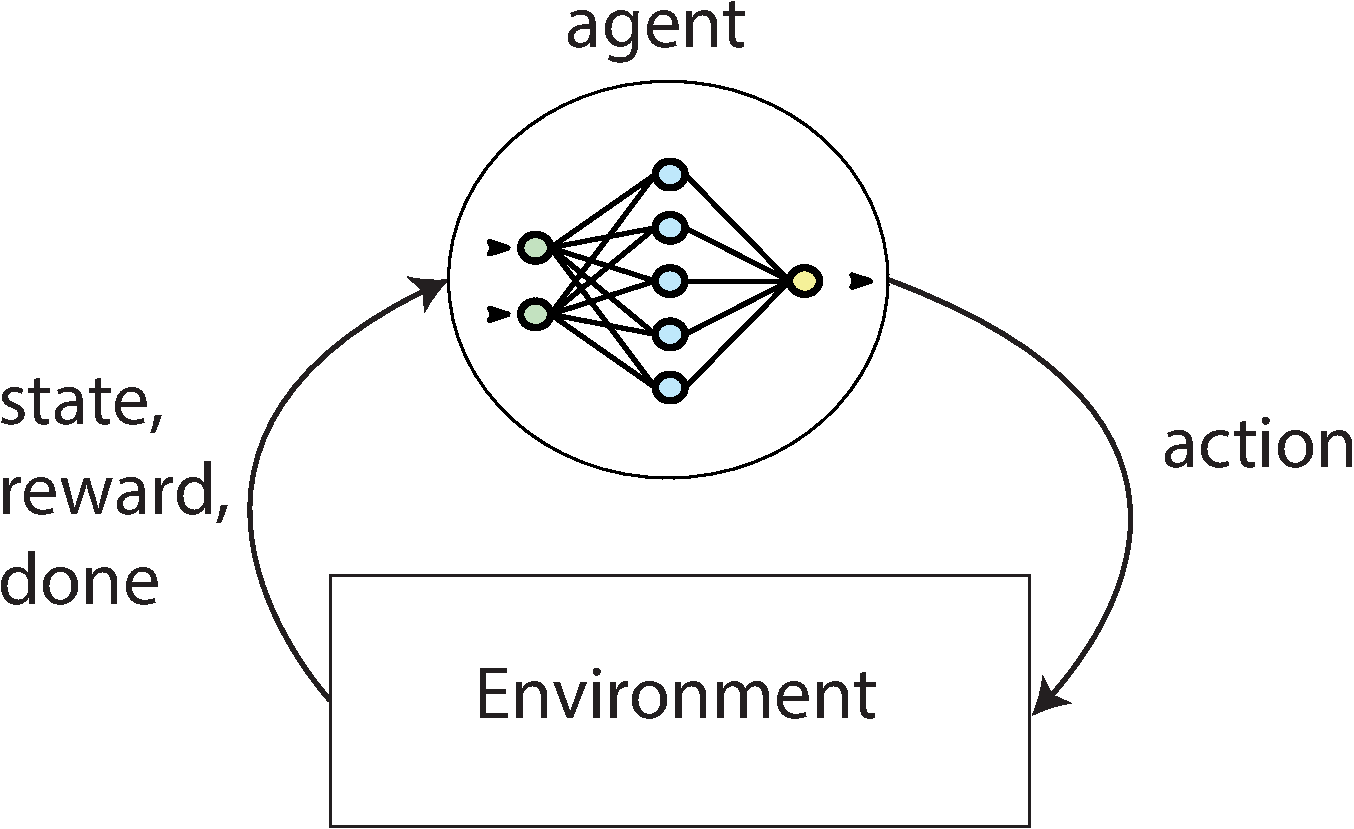
\includegraphics[width=0.6\linewidth]{images/rl_setting}
    }
    \caption{Ваимодействик RL агента и среды}\label{fig:rl_setting}
\end{figure}

Математическое ожидание суммарной дисконтированной награды вычисляется по траекториям при условии текущей стратегии агента по формуле: 

\[
E_{\tau \sim \pi(\theta)} [G(\tau)] = E_{\tau \sim \pi(\theta)} [R_0 + \gamma R_{1} + \gamma ^ 2 R_{2} + ...] = E_{\tau \sim \pi(\theta)} [\sum_{t=0}^{T - 1} \gamma ^t R_{t}]
\]

Взаимодействие агента и среды рассматривается в предположении марковского процесса принятия решений. С учетом этого предположения оптимальная стратегия агента зависит только от текущего состояния среды что позволяет использовать уравнение оптимальности Беллмана выражающее связь между оптимальной стратегией в двух последовательных состояниях среды $s$ и $s'$

\[
	V^*(s) = \max_{a \in \mathcal{A}} E(r_{t + 1}(s, a, s') + \gamma V^*(s_{t + 1}))
\]
где $V^*(s)$ (V-функция) - математическое ожидание суммарной дисконтированной награды в состоянии $s$ при условии оптимальной стратегии, а $\gamma$ - коэффициент дисконтирования. Эквивалентно уравнение Беллмана можно записать следующим образом: 

\[
	Q^*(s, a) = E(r_{t + 1}(s, s', a) + \max_{a \in \mathcal{A}} \gamma Q^*(s_{t + 1}, a))
\]

где $Q^*(s, a)$ (Q-функция) - математическое ожидание суммарной дисконтированной награды в состоянии $s$ при условии действия $a$ и следовании оптимальной стратегии в следующем состоянии $s'$.

Далее рассматриваются основные алгоритмы применяемые в машинном обучении с подкреплением. Условно их можно разделить на два больших класса <<off-policy>> и <<on-policy>> методы. Off-policy методы основываются на идее аппроксимации Q-функции c использованием метода временных разностей. Такие методы могут использовать данные полученные стратегией сколь угодно сильно отличающейся от текущей стратегии. Благодаря этому off-policy методы обычно требуют меньше данных, но более подвержены численным не стабильностям при обучении. С другой стороны on-policy методы основываются на идее максимизации суммарной ожидаемой награды благодаря чему они численно более стабильны, но требуют существенно больше данных для обучения. 

Затем рассматриваются подходы применяемые в обучнии с подкреплением в задачах с разреженной наградой. В таких задачах вероятность того, что агент со случайной стратегией найдет не нулевую награду и тем самым получит положительный сигнал для обучения пренебрежимо мала. В этом случае используются подходы называемые внутренней мотивацией (intrinsic motivation). Общая идея данных подходов заключается в том, чтобы давать агенту награды за достижение состояний в которых он раньше не был, что позволит эффективно исследовать среду. 

Последним из подходов используемых в обучении с подкреплением расматривается иерархическое обучение с подкреплением. Данный класс методов направлен на построение иерархии навыков в которой стратегии нижнего уровня решают подзадачи используемые следующими стратегиями для решения более общих задач. 

В конце главы рассматривается применение методов глубокого машинного обучения с подкреплением в задачах управления робототехническими устройствами. По сравнению с классическими методами основанными на обратной кинематике алгоритмы машинного обучения способны самостоятельно адаптироваться к параметрам робота и соответственно работать в условиях когда эти параметры точно не известны или значения получаемые при измерении этих параметров имеют большой разброс. 

\underline{\textbf{Вторая глава}} посвящена разработке метода автоматической настройки оптического интерферометра Маха-Цендера по изображениям с камеры методом машинного обучения с подкреплением. В начале описываются физические принципы работы оптического интерферометра. Затем приводится построенная на основе этих принципов компьютерная модель позволяющаяя моделировать изображения получаемые на камере оптического интерферометра при произвольном расположении оптических элементов - зеркал и линз интерферометра. Примеры изображений полученных с помощью разработанной программы приведены на рисунке \ref{fig:visib_expl}. 

\begin{figure}[ht]
    \centerfloat{
        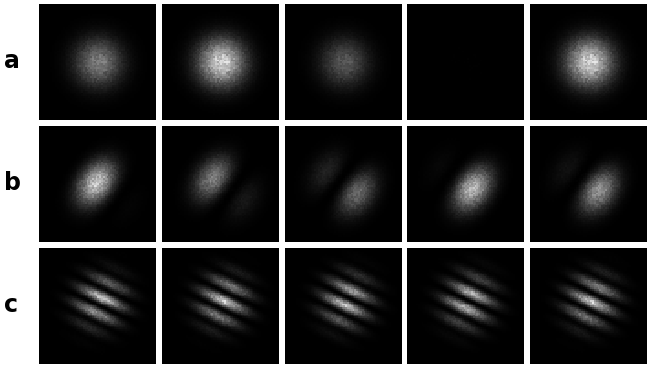
\includegraphics[width=0.8\linewidth]{images/visib_expl}
    }
    \caption{
    Изображения интерференции для различных положения зеркал полученные с помощью симуляционной программы. (a) Идеально настроенный интерферометр, видность = 1; (b) Слабо расстроенный интерферометр, видность = 0.3; (c) Сильно расстроенный интерферометр, видность = 0.0026. Изображения слева на право соответствуют различным моментам времени.}
\label{fig:visib_expl}
\end{figure}

Далее задача настройки интерферометра сводится к марковскому процессу принятия решений и обучению с подкреплением. Общая схема интерферометра настраеваемого алгоритмом изображена на рисунке \ref{fig:interf_scheme}. На ней RL агент управляет линзой $lens 2$ и светоделителями $bs1$ и $bs2$. 

\begin{figure}[ht]
    \centerfloat{
        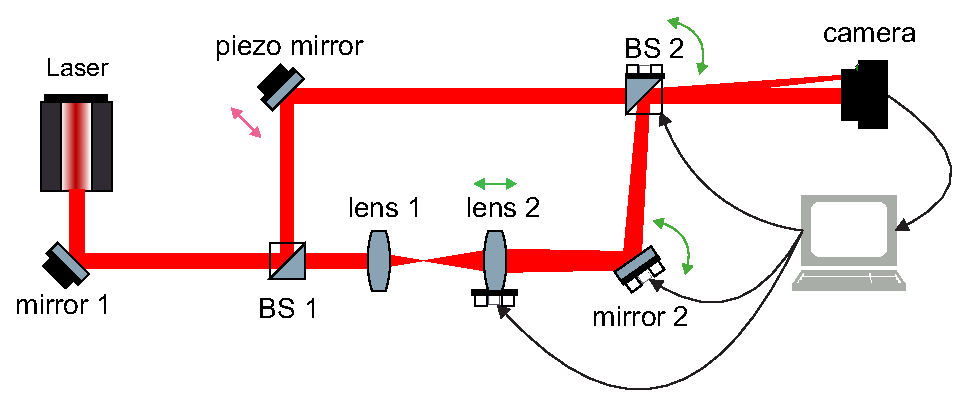
\includegraphics[width=0.8\linewidth]{images/interferobot_scheme}
    }
    \caption{Ваимодействик RL агента и среды}\label{fig:interf_scheme}
\end{figure}

Далее рассматриваются подходы к определению пространства действий агента и функции награды. Обосновывается использование в качестве нагады функции $r = vis - log(1 - vis)$, где $vis$ - видность интерференционной картины, основная метрика качества настройки интерферометра. Приводятся результаты обучения агента в симуляции с использованием дисктного и непрерывного пространств действий. Затем рассматриваются рандомизации использованные при обучении агентов в симуляции для успешного переноса на экспериментальную установку. В заключении приводятся результаты тестирования агентов на экспериментальной установке, сравнение качества настройки интерферомета с человеком и анализ стратегии используемой агентами при настройке интерферометра. 

\begin{figure}[ht]
    \centerfloat{
        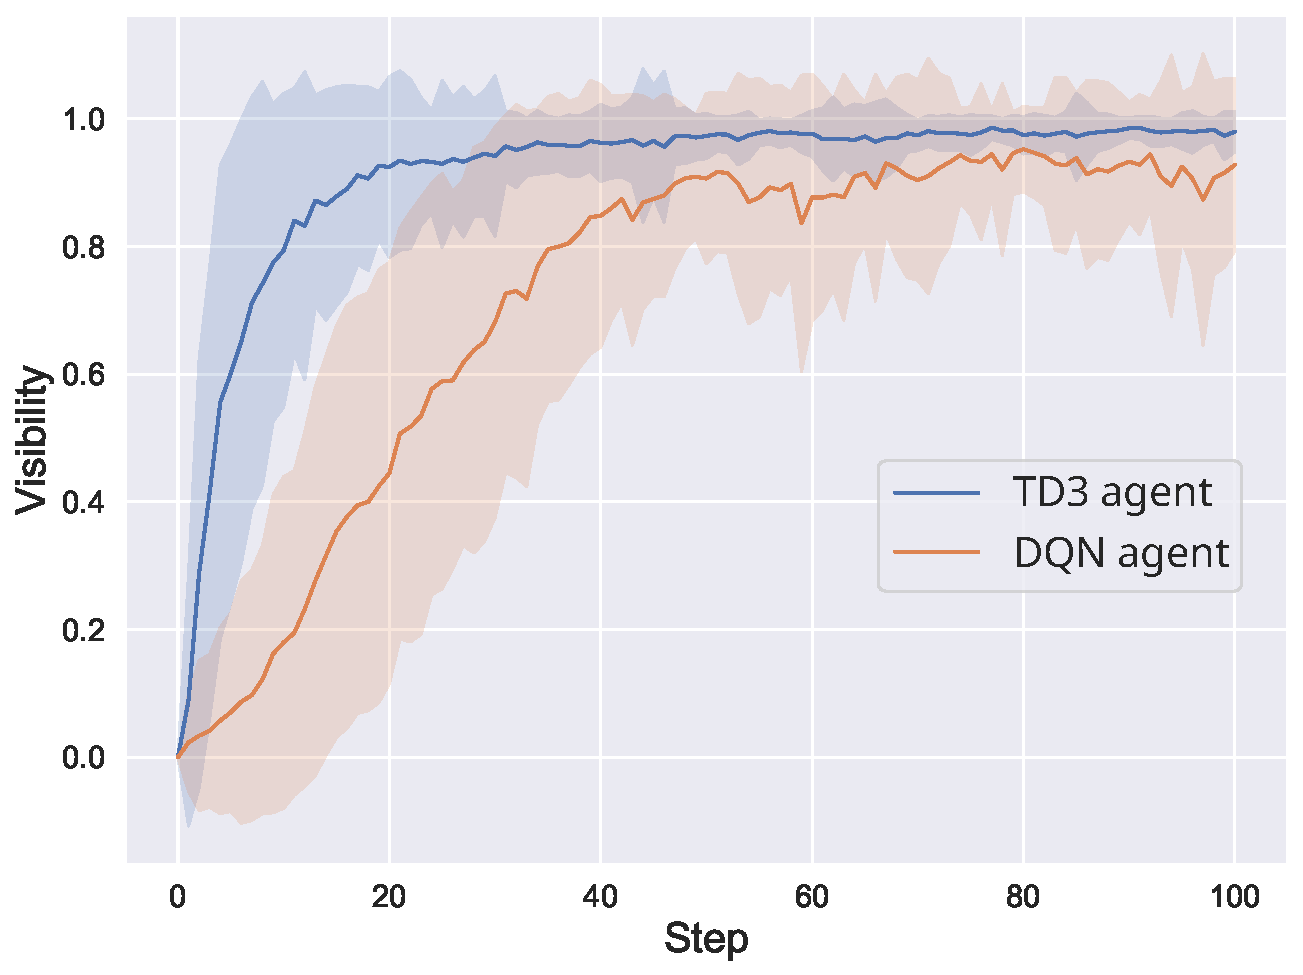
\includegraphics[width=0.8\linewidth]{images/dqn_vs_td3}
    }
    \caption{Тестирование агентов на экспериментальной установке}\label{fig:interf_test}
\end{figure}

Результаты тестирования приведены на рисунке \ref{fig:interf_test}. По оси абсцисс отложен номер шага настройки, по оси ординат отложена достигнутая видность. Результаты усреднены по 100 эпизодам. Из рисунка \ref{fig:interf_test} видно, что оба метода достигают хорошего значения видности интерференционной картины, но агент TD3 использующий непрерывное пространство действий работает быстрее и достигает лучшей видности чем DQN агент использующий дискретное пространство действий. 


Разультаты работы опубликованы в статьях \cite{confbib1, confbib2} на ведущих научных конференциях <<Neural information processing systems (NeurIPS)>> и <<Conference on Robot Learning (CoRL)>> также на программу автоматической настройки интерферометра по изображениям с камеры с импользованием машинного обучения получен РИД \cite{progbib1}.

\underline{\textbf{Третья глава}} посвящена исследованию методов машинного обучения с подкреплением для использования в среде Nethack. Среда Nethack основанна на одноименной игре и предложена в качестве теста для алгоритмов машинного обучения в 2020 году \cite{nethack}. В этой игре агент путешествует по процедурно генерируемому подземелью. Игра имеет ascii интерфейс изображенный на рисунке \ref{fig:nethack}.

\begin{figure}[ht]
    \centerfloat{
        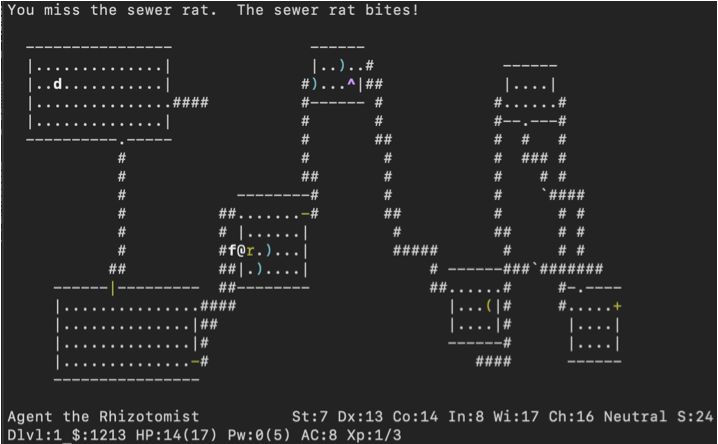
\includegraphics[width=0.8\linewidth]{images/nethack}
    }
    \caption{Игра Nethack}\label{fig:nethack}
\end{figure}

Основную сложность для алгоритмов обучения с подкреплением составляют сочетание различных типов данных в состоянии (изображения, текстовые описания, табличные данные), редкая функция награды и комбинаторно большое пространство действий. Далее приводится разработанный метод сочетающий в себе машинное обучение с подкреплением, алгоритмы навигации на графах и алгоритмы основанные на экспертных знаниях. 

\SetKwComment{Comment}{/* }{ */}
\SetKw{Continue}{continue}

\begin{algorithm}
\caption{RAPH algorithm}\label{alg:one}
\KwData{view\_distance, agent}
$state \gets env.reset()$\;
$done \gets False$\;

\While{not done}{
  action\_queue = senses.update(state)\;

  \If{action\_queue} {
   state, reward, done, info = env.step(action\_queue) \Comment*[r]{We have a prompt to response}
   \Continue
  }

  level.update(state)\;
  inventory.update(state)\;
  hero.update(state)\;
  \eIf{monster\_distance \textless view\_distance}{
    action\_queue = agent.act(preprocessed\_state)\;
  }{
    action\_queue = first\_fit(non-rl-actions)\Comment*[r]{Select non-rl action on first-fit basis}
  }
  state, reward, done, info = env.step(action\_queue)\;
}

\label{alg:raph}
\end{algorithm}

Данный подход позволил превзойти остальные подходы с использованием обучения с подкреплением в этой задаче. Результаты были опубликованы на одной из ведущих конференции по машинному обучению NeurIPS в рамках трека посвященного соревнованиям \autocite{confbib3}.


\FloatBarrier
\pdfbookmark{Заключение}{conclusion}                                  % Закладка pdf
В \underline{\textbf{заключении}} приведены основные результаты работы, которые заключаются в следующем:
%% Согласно ГОСТ Р 7.0.11-2011:
%% 5.3.3 В заключении диссертации излагают итоги выполненного исследования, рекомендации, перспективы дальнейшей разработки темы.
%% 9.2.3 В заключении автореферата диссертации излагают итоги данного исследования, рекомендации и перспективы дальнейшей разработки темы.
\begin{enumerate}
  \item Была разработанна компьютерная модель оптического интерферометра Маха-Цендера. Процесс настройки интерферометра был представлен в виде марковского процесса принятия решений на основании которого была разработана среда для обучения агентов машинного обучения с подкреплением по настройке оптического интерферометра. 
  \item На основе среды были разработаны методы основанные на обучении с подкреплением, которые позволили выучить алгоритм настройки интерферометра по изображениям с камеры. 
  \item Разработанные методы были успешно протестированы при настройке экспериментальной установки интерферометра. 
  \item Был разработан метод включающий в себя обучения с подкреплением для управлением виртуальным агентом в среде Nethack. 
\end{enumerate}

\newpage


\pdfbookmark{Литература}{bibliography}                                % Закладка pdf

\ifdefmacro{\microtypesetup}{\microtypesetup{protrusion=false}}{} % не рекомендуется применять пакет микротипографики к автоматически генерируемому списку литературы
\urlstyle{rm}                               % ссылки URL обычным шрифтом
\ifnumequal{\value{bibliosel}}{0}{% Встроенная реализация с загрузкой файла через движок bibtex8
    \renewcommand{\bibname}{\large \bibtitleauthor}
    \nocite{*}
    \insertbiblioauthor           % Подключаем Bib-базы
    %\insertbiblioexternal   % !!! bibtex не умеет работать с несколькими библиографиями !!!
}{% Реализация пакетом biblatex через движок biber
    % Цитирования.
    %  * Порядок перечисления определяет порядок в библиографии (только внутри подраздела, если `\insertbiblioauthorgrouped`).
    %  * Если не соблюдать порядок "как для \printbibliography", нумерация в `\insertbiblioauthor` будет кривой.
    %  * Если цитировать каждый источник отдельной командой --- найти некоторые ошибки будет проще.
    %
    %% authorvak
    \nocite{vakbib1}%
    \nocite{vakbib2}%
    %
    %% authorwos
    \nocite{wosbib1}%
    %
    %% authorscopus
    \nocite{scbib1}%
    %
    %% authorpathent
    \nocite{patbib1}%
    %
    %% authorprogram
    \nocite{progbib1}%
    %
    %% authorconf
    \nocite{confbib1}%
    \nocite{confbib2}%
    \nocite{confbib3}%
    %
    %% authorother
    \nocite{bib1}%
    \nocite{bib2}%

    \ifnumgreater{\value{usefootcite}}{0}{
        \begin{refcontext}[labelprefix={}]
            \ifnum \value{bibgrouped}>0
                \insertbiblioauthorgrouped    % Вывод всех работ автора, сгруппированных по источникам
            \else
                \insertbiblioauthor      % Вывод всех работ автора
            \fi
        \end{refcontext}
    }{
        \ifnum \totvalue{citeexternal}>0
            \begin{refcontext}[labelprefix=A]
                \ifnum \value{bibgrouped}>0
                    \insertbiblioauthorgrouped    % Вывод всех работ автора, сгруппированных по источникам
                \else
                    \insertbiblioauthor      % Вывод всех работ автора
                \fi
            \end{refcontext}
        \else
            \ifnum \value{bibgrouped}>0
                \insertbiblioauthorgrouped    % Вывод всех работ автора, сгруппированных по источникам
            \else
                \insertbiblioauthor      % Вывод всех работ автора
            \fi
        \fi
        %  \insertbiblioauthorimportant  % Вывод наиболее значимых работ автора (определяется в файле characteristic во второй section)
        \begin{refcontext}[labelprefix={}]
            \insertbiblioexternal            % Вывод списка литературы, на которую ссылались в тексте автореферата
        \end{refcontext}
        % Невидимый библиографический список для подсчёта количества внешних публикаций
        % Используется, чтобы убрать приставку "А" у работ автора, если в автореферате нет
        % цитирований внешних источников.
        \printbibliography[heading=nobibheading, section=0, env=countexternal, keyword=biblioexternal, resetnumbers=true]%
    }
}
\ifdefmacro{\microtypesetup}{\microtypesetup{protrusion=true}}{}
\urlstyle{tt}                               % возвращаем установки шрифта ссылок URL
